\begin{equation}
    \begin{gathered}
        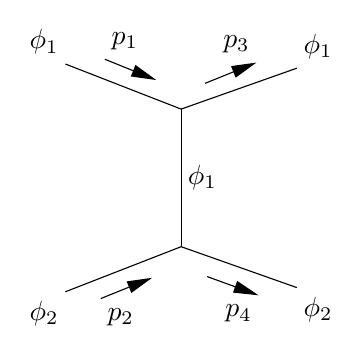
\begin{tikzpicture}[x=0.75pt,y=0.75pt,yscale=-1,xscale=1]
            %uncomment if require: \path (0,300); %set diagram left start at 0, and has height of 300
            
            %Straight Lines [id:da968688619535284] 
            \draw    (279.45,82.74) -- (223.71,102.45) ;
            %Straight Lines [id:da6740832290961962] 
            \draw    (167.97,80.74) -- (223.71,102.45) ;
            %Straight Lines [id:da7441488382972461] 
            \draw    (186.98,78.45) -- (209.85,87.7) ;
            \draw [shift={(211.71,88.45)}, rotate = 202.02] [fill={rgb, 255:red, 0; green, 0; blue, 0 }  ][line width=0.08]  [draw opacity=0] (12,-3) -- (0,0) -- (12,3) -- cycle    ;
            %Straight Lines [id:da6192843702040114] 
            \draw    (258.14,80.78) -- (235.27,90.03) ;
            \draw [shift={(259.99,80.03)}, rotate = 157.98] [fill={rgb, 255:red, 0; green, 0; blue, 0 }  ][line width=0.08]  [draw opacity=0] (12,-3) -- (0,0) -- (12,3) -- cycle    ;
            %Straight Lines [id:da5061127031046193] 
            \draw    (223.71,102.45) -- (223.71,168.74) ;
            %Straight Lines [id:da9802616713197088] 
            \draw    (279.45,188.45) -- (223.71,168.74) ;
            %Straight Lines [id:da37815238333918666] 
            \draw    (167.97,190.45) -- (223.71,168.74) ;
            %Straight Lines [id:da8760769937547084] 
            \draw    (184.98,193.74) -- (207.85,184.49) ;
            \draw [shift={(209.71,183.74)}, rotate = 517.98] [fill={rgb, 255:red, 0; green, 0; blue, 0 }  ][line width=0.08]  [draw opacity=0] (12,-3) -- (0,0) -- (12,3) -- cycle    ;
            %Straight Lines [id:da297806715922456] 
            \draw    (259.11,191.47) -- (236.27,183.15) ;
            \draw [shift={(260.99,192.15)}, rotate = 200] [fill={rgb, 255:red, 0; green, 0; blue, 0 }  ][line width=0.08]  [draw opacity=0] (12,-3) -- (0,0) -- (12,3) -- cycle    ;
            
            % Text Node
            \draw (165.97,77.34) node [anchor=south east] [inner sep=0.75pt]    {$\phi _{1}$};
            % Text Node
            \draw (165.97,193.85) node [anchor=north east] [inner sep=0.75pt]    {$\phi _{2}$};
            % Text Node
            \draw (188.98,75.05) node [anchor=south west] [inner sep=0.75pt]    {$p_{1}$};
            % Text Node
            \draw (186.98,197.14) node [anchor=north west][inner sep=0.75pt]    {$p_{2}$};
            % Text Node
            \draw (225.71,135.59) node [anchor=west] [inner sep=0.75pt]    {$\phi _{1}$};
            % Text Node
            \draw (257.99,76.63) node [anchor=south east] [inner sep=0.75pt]    {$p_{3}$};
            % Text Node
            \draw (258.99,195.55) node [anchor=north east] [inner sep=0.75pt]    {$p_{4}$};
            % Text Node
            \draw (281.45,79.34) node [anchor=south west] [inner sep=0.75pt]    {$\phi _{1}$};
            % Text Node
            \draw (281.45,191.85) node [anchor=north west][inner sep=0.75pt]    {$\phi _{2}$};
            \end{tikzpicture}            
    \end{gathered} \eqqcolon \ii \mathcal{M}_{t1} = \frac{\ii}{(p_1 - p_3)^2 + \ii 0^+} (\ii g)^2 = - \ii \frac{g^2}{t + \ii 0^+},
\end{equation}